% Solutions des questions de dépannage du chapitre 6
\section{Questions}
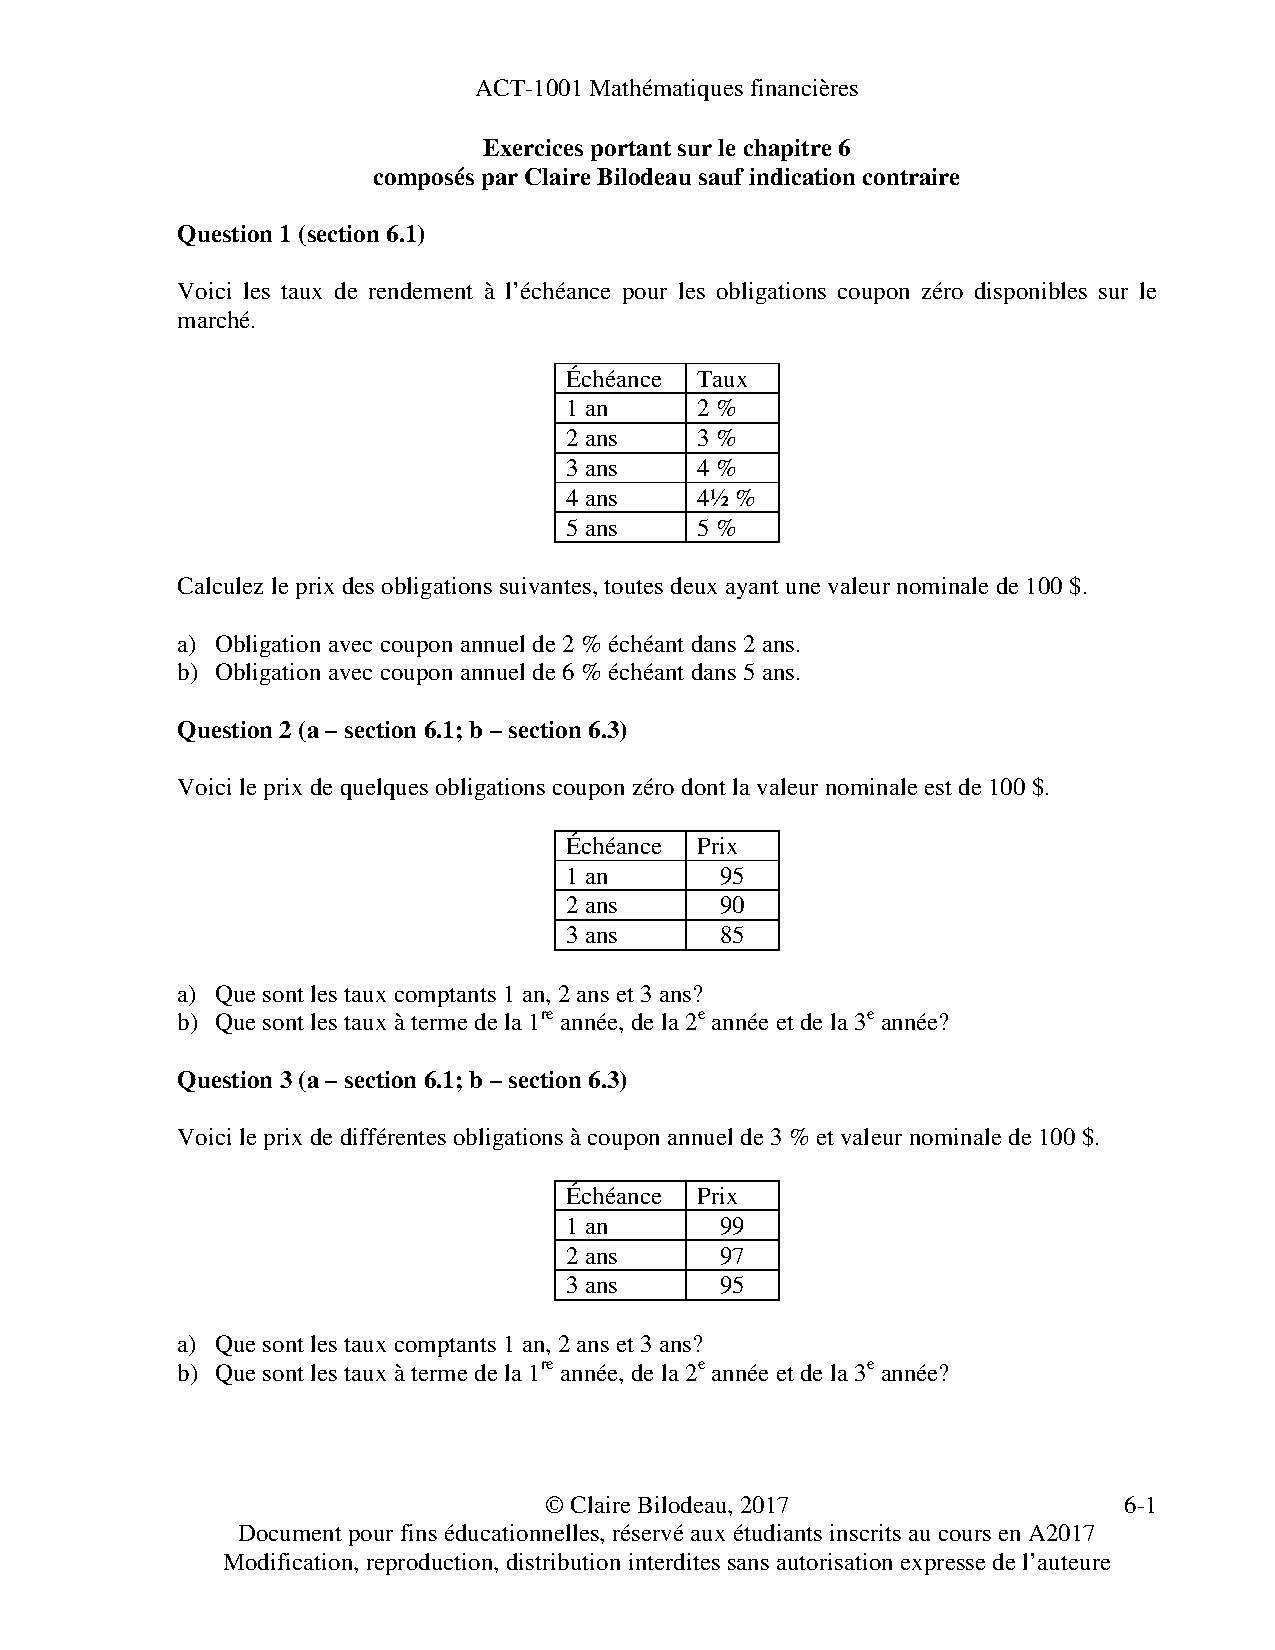
\includepdf[pages = 1-]{questions/depanchap6.pdf}

\section{Solutions}
\begin{enumerate}
  \item % Question 1
  Pour cette question, on nous donne les \emph{spot-rate} pour des obligations
  zéro-coupon venant à échéance dans 1 à 5 ans. Donc, on peut voir les obligations
  qu'on nous demande de calculer en a) et b) comme plusieurs obligations \emph{zéro-coupon}
  avec des échéances différentes (pour chaque coupon.)
  \begin{enumerate}[label=\alph*)]
    \item Pour cette obligation, c'est comme si on avait 2 obligations zéro-coupon :
    une avec une échéance dans 1 an, et l'autre avec une échéance dans 2 ans. Alors,
    \begin{align*}
      P     & = P(0,1) + P(0,2) \\
      \\
      P(0,1)& = Fr(1+s_0(1))^{-1} \\
            & = (100 \cdot 0,02)(1+0,02)^{-1} \\
            & = 1,96 \\
      \\
      P(0,2)& = F(1+r)(1+s_0(2))^{-2} \\
            & = 102(1,03)^{-2} \\
            & = 96,14478273 \\
      \\
      P     & = 1,960784314 + 96,14478273 \\
            & = 98,10556704 \\
    \end{align*}
    \item Même principe pour le b), mais avec 5 obligations... c'est donc beaucoup
    plus long :
    \begin{align*}
      P   & = P(0,1) + P(0,2) + P(0,3) + P(0,4) + P(0,5) \\
          & = Fr(1+s_0(1))^{-1} + Fr(1+s_0(2))^{-2} + Fr(1+s_0(3))^{-3} \\
          & + Fr(1+s_0(4))^{-4} + F(1+r)(1+s_0(5))^{-5} \\
          & = 6(1,02)^{-1} + 6(1,03)^{-2} + 6(1,04)^{-3} + 6(1,045)^{-4} + 106(1,05)^{-5} \\
          & = 104,9570483 \\
    \end{align*}
  \end{enumerate} % fin question 1
  \item Si l'on connaît le prix des obligations \emph{zéro-coupon} avec des échéances
  données, nous somme capable d'isoler $s_0(n)$.
  \begin{enumerate}[label=\alph*)]
    \item % a)
    \begin{align*}
      P(0,1)  & = F(1+s_0(1))^{-1} \\
      s_0(1)  & = \frac{F}{P(0,1)} - 1 \\
              & = \frac{100}{95} -1 \\
              & = 0,052631579 \\
      \\
      P(0,2)  & = F(1+s_0(2))^{-2} \\
      s_0(2)  & = \frac{F}{P(0,2)} - 1 \\
              & = \left( \frac{100}{90} \right)^{1/2} -1 \\
              & = 0,054092553 \\
      \\
      P(0,3)  & = F(1+s_0(3))^{-3} \\
      s_0(3)  & = \frac{F}{P(0,3)} - 1 \\
              & = \left( \frac{100}{85} \right)^{1/3} -1 \\
              & = 0,055667192 \\
    \end{align*}
    \item Les taux à termes (\emph{Forward rate}) sont des taux pour lesquels, en
    fonction des taux \emph{spot} en vigueur, le rendement que l'on peut faire
    d'une année à l'autre dans le futur.
    \p
    La formule générale pour trouver un taux $i_o(n)$ est :
    \begin{displaymath}
      i_0(n-1,n) = \frac{(1+s_0(n))^n}{(1+s_0(n-1))^{n-1}} -1
    \end{displaymath}
    Alors,
    \begin{align*}
      i_0(0,1)  & = s_0(1) \\
                & = 0,052631579 \\
      \\
      i_0(1,2)  & = \frac{(1+s_0(2))^2}{(1+s_0(1))^1} -1  \\
                & = \frac{(1,054092553)^2}{0,052631579} \\
                & = 0,0555555555 \\
      \\
      i_0(2,3)  & = \frac{(1+s_0(3))^3}{(1+s_0(2))^2} \\
                & = \frac{(1+0,055667192)^3}{(1+0,054092553)^2} \\
                & = 0,058823529 \\
    \end{align*}
  \end{enumerate} % fin question 2
  \item Ici la question est posée différente. Les prix donnés correspondent à
  des obligations normales \underline{avec coupon}.
  \p
  Il faut donc commencer par isoler $s_0(1)$ avec le prix de l'obligation qui
  va être échue dans 1 an, puis isoler $s_0(2)$ sachant qu'on connaît $s_0(1)$, etc...
  \begin{enumerate}[label=\alph*)]
    \item Pour l'obligation à échéance 1 ans
    \begin{align*}
      P       & = F(1+r)(1+s_0(1))^{-1} \\
      s_0(1)  & = \frac{F(1+r)}{P} -1 \\
              & = \frac{100(1,03)}{99}  -1\\
              & = 0,0404040404 \\
      \text{l'obligation 2 ans ...}\\
      P       & = Fr(1+s_0(1))^{-1} + F(1+r)(1+s_0(2))^{-2} \\
      s_0(2)  & = \left( \frac{P - Fr(1+s_0(1))^{-1}}{F(1+r)} \right)^{-1/2} - 1 \\
              & = \left( \frac{97 - 3(1,0404040404)^{-1}}{103} \right)^{-1/2} - 1 \\
              & = 0,046130146 \\
      \text{l'obligation 3 ans ...}\\
      P       & = Fr(1+s_0(1))^{-1} + Fr(1+s_0(2))^{-2} + F(1+r)(1+s_0(3))^{-3} \\
      s_0(2)  & = \left( \frac{P - Fr(1+s_0(1))^{-1} - Fr(1+s_0(2))^{-2}}{F(1+r)} \right)^{-1/3} - 1 \\
              & = \left( \frac{97 - 3(1,0404040404)^{-1}- 3(1,046130146)^{-2}}{103} \right)^{-1/3} - 1 \\
              & = 0,048431327 \\
    \end{align*}
    \item pour trouver les taux \emph{forward}, on effectue exactement les mêmes
    calculs qu'au numéro 2 ci-haut :
    \begin{align*}
      i_0(0,1)  & = 0,0404040404 \\
      i_0(1,2)  & = 0,051887767 \\
      i_0(2,3)  & = 0,053048886 \\
    \end{align*}
  \end{enumerate} % Fin du numéro 3
  \item On nous donne dans la   question nos $i_0(n-1,n)$, il faut connaître
  l'entité suivante :
  \begin{displaymath}
    (1+s_0(n))^n = (1 + i_0(0,1) \times (1+i_0(1,2)) \times ... \times (1+i_0(n-1,n)))
  \end{displaymath}
  On n'a donc pas besoin de convertir nos taux \emph{forward}, simplement
  successivement les coupons des obligations avec les bons taux.
  \begin{enumerate}[label=\alph*)]
    \item
    \begin{align*}
      P     & = Fr(1+i_0(0,1))^{-1} + F(1+r)(1+i_0(0,1))(1+i_0(1,2)) \\
            & = 2(1,025)^{-1} + 102(1,025)^{-1}(1,03)^{-1} \\
            & = 98,5165001184 \\
    \end{align*}
    \item Même principe, mais les calculs se rallongent ...
    \begin{align*}
    P   & = \sum_{k=1}^5 Fr \prod_{u=1}^k (1+i_0(u-1,u))^{-1} + \frac{100}{\prod_{u=1}^5 (1+i_0(u-1,u))} \\
        & = \frac{6}{1,025} + \frac{6}{(1,025)(1,03)} + ... \\
    P   & = 111,567160440 \\
    \end{align*}
  \end{enumerate} % Fin du numéro 4
\item
\begin{enumerate}
  \item On nous demande seulement de calculer notre $i_(3,4)$ sachant qu'on connaît
  $s_0(4)$ et $s_0(4)$.
  \p
  \begin{align*}
    i_0(3,4)  & = \frac{(1+s_0(4))^4}{(1+s_0(3))^3}-1 \\
              & = \frac{(1,07)^4}{(1,08)^3} -1 \\
              & = 0,040552134 \\
  \end{align*}

  \item Si quelqu'un nous offre un taux inférieur au taux \emph{forward} auquel
  on pourrait s'engager, alors l'économie conrrespond à la différence entre le
  taux $i_(3,4)$ trouvé en a) et le taux $i^*$ offert:
  \begin{align*}
    \text{économies}  & = |i_0(3,4) - i^*| \times 30\ 000 \$ \\
                      & = (0,040552134 - 0,0375) \times 30000 \\
                      & = 91,56402\$ \\
  \end{align*}
\end{enumerate} % fin du numéro 5
\end{enumerate}
